% This document is for a tutorial video
%https://www.overleaf.com/learn/latex/LaTeX_video_tutorial_for_beginners_(video_1)

% All \ are Laytek commands

\documentclass[letterpaper,12pt]{article}  % Tells what type of document you want to make. Article is useful for scientific journal.
% https://www.youtube.com/watch?v=CxOCIfQhFmI&ab_channel=ShareLaTeX
% If you want a longer option you can use book or Journal class
% Can add chapters, split up documents into multiple files
\usepackage{tabularx} % extra features for tabular environment

\usepackage[utf8]{inputenc}  % lets you use accented UTF8 characters
\usepackage{amsmath}  % amsmath for more math options
\usepackage{graphicx}  % graphics package
\graphicspath{{Images/}}  % adds image path for putting in folder
% Bibtek is included automatically
%\usepackage[round]{natbib} % helps customize references
\usepackage[margin=1.25in,letterpaper]{geometry} % decreases margins
\usepackage{cite} % takes care of citations
\usepackage[final]{hyperref} % adds hyper links inside the generated PDF file
\hypersetup{
	colorlinks=true,       % false: boxed links; true: colored links
	linkcolor=blue,        % color of internal links
	citecolor=blue,        % color of links to bibliography
	filecolor=magenta,     % color of file links
	urlcolor=blue
}
\usepackage{blindtext}
\usepackage{fancyhdr}
\usepackage{enumitem}
\usepackage{sectsty}

\sectionfont{\fontsize{12}{12}\selectfont}

% \usepackage{natbib}  % Used for fancier biliography/citations
% \bibliographystyle{plainnat}  % the style setup
%\setlist{itemsep=1pt,leftmargin=*}

% Inserts key turns on and off text insert mode


%++++++++++++++++++++++++++++++++++++++++
% Decided not to do traditional title because it took to much space
% Using fancy header formatting https://www.overleaf.com/learn/latex/headers_and_footers#Standard_page_styles

\pagestyle{fancy}
\fancyhf{}
\rhead{CSE 701 -  Final Project - NPC Racer \newline Brendan Fallon}
\lhead{\today{}}  % April 14, 2021
\rfoot{Page \thepage}
\lfoot{}

\title{ % Make subtitle lines with \\
    NPC Racer \\
    \large A Comparative Analysis of Game Agent Pathfinding Algorithms \\
    CAS 701 - Foundations of Modern Scientific Programming - \\
    Final Project}
\date{\today{}} %Wednesday, April 14, 2021
\author{Brendan Fallon}

%++++++++++++++++++++++++++++++++++++++++

% This is all preamble

\begin{document}  % Always need begin and end

\maketitle  % This makes the title of the document from the preamble

\tableofcontents  % makes a table of contents

\section{Introduction to the Project}
\subsection{Background}
Non-playable characters (NPCs) or video game agents are critical elements for immersing players into a world \cite{noauthor_toby_nodate}. My research focuses on the believability of agents when incorporating cognitive elements such as emotion. To show behaviour that looks believable, agents need a controlling system to take in input from the world and react accordingly, such as reacting to player input. To aid programming agents for my research and others I’d like to create a domain-specific language (DSL) in the Eclipse Modelling Framework (EMF) based on specifying the control of NPCs. That way, a character designer could specify the way an agent should behave without having to deal with the programming details. The model produced by the character designer could be then given to a game programmer to implement with help of code generation. This domain-specific language would provide another level of abstraction to more easily implement video game agents.

\subsection{Decision tree control logic}
There are many systems to control game agent's behaviour including decision trees, behaviour trees, finite state machines (FSMs), hierarchical finite state-machines (HFSMs), or goal-oriented action planning (GOAP) \cite{ai_and_games_behaviour_2019}. Often these methods are tedious, time-consuming, and undergo massive complexity increases as the number of behaviours increases. I wanted to keep my scope small so I started with the most basic control scheme, binary decision trees, which is essentially conditional logic. These trees are simplistic but can be easily restructured into behaviour trees, which are used much more useful and in the video game industry \cite{ai_and_games_behaviour_2019}.

Decision trees are composed of decision nodes and leaf nodes. Decision nodes contain conditional logic that should result in true/false or yes/no answers. These help direct the control logic down the tree. They also have two children nodes, hence a binary tree, connected by the edges of true or false. Leaf nodes are the leaves of the tree and only contain the action or behaviour to be performed. An example of a decision tree can be seen in figure \ref{fig:decisiontree}.

\begin{figure}[h]  % h for here, p for separate page, b\t, or !
    \centering  % centers the figure in the page
    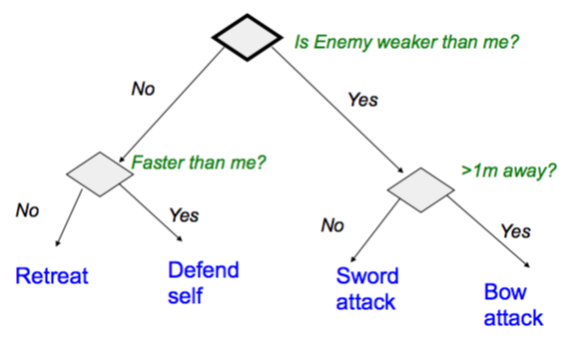
\includegraphics[width = 8 cm ]{DecisionTree.png}
    \caption{A binary decision tree showing simple behaviour control for a game agent.}
    \label{fig:decisiontree}
\end{figure}

\subsection{DSL Integration & Features}
Agents don’t live on their own and interact based on the state of the world. As such, the model will also have to include other game-world elements. To keep it simple I decided to start with a simple location structure, which contains an agent and other adjacent locations. A player can be incorporated by simply giving an agent a "layerinput method and a specific player controller tree. For abstraction purposes, all these game elements often incorporate into a larger game engine. One of the most popular options is the Unity game engine \cite{technologies_unity_nodate}. However, code integration into an actual game is outside the scope of this project so I’ll be starting with generating code into a programming language I’m very familiar with such as Python.

With the limited scope, some of the minimum features the DSL would include:
1)	 Modelling agents and locations in a graphical editor
2)	Authoring NPC behaviours using decision trees
3)	Generating Python code

All these features could be extended to make more advanced tooling such as behaviour tree controllers, specifying items, specifying agent goals (i.e. NPC wants shiny rock), and generating code for scripting in Unity.



\section{Metamodel Abstract Syntax}
\subsection{Metamodel}
Having defined the agentgame metamodel in Emfatic the class diagram of the metamodel is seen in figure \ref{fig:metamodel}. The metamodel is composed of 5 classes plus the encapsulating game class which allows any number of the game elements to be made. The location, agent, decisiontree, decisionnode, and leafnode class are all directly connected with associations or composition relationships.

\begin{figure}[h]  % h for here, p for separate page, b\t, or !
    \centering  % centers the figure in the page
    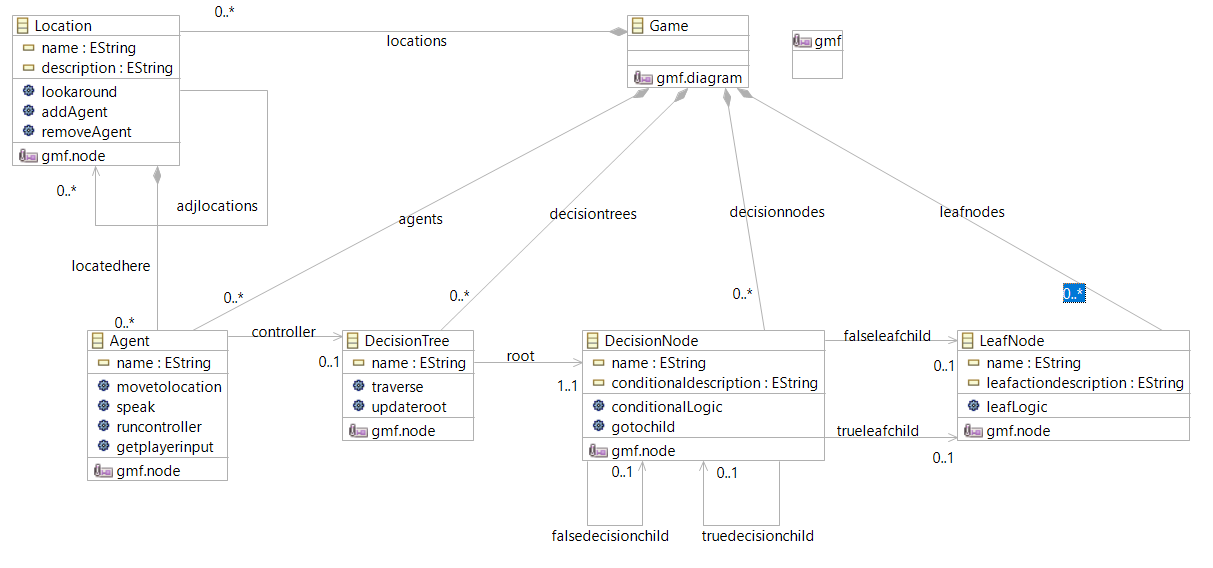
\includegraphics[width = 16 cm ]{Agentgame MetaModel Class Diagram.png}
    \caption{The agentgame metamodel class diagram.}
    \label{fig:metamodel}
\end{figure}


\subsection{Alternative Designs}
Alternative designs could have included much more advanced controllers such as finite-state machines, behaviour trees, or goal-oriented action planning. I was advised that state machines are tricky to the metamodel. Also, I wanted to start with the simplest metamodel possible and then build out the technology from there in an iterative fashion. I believe this iterative design style helps learn the technology involved much faster and discover any fundamental flaws before building a complex structure. This “keep it simple” design philosophy also applies to the scope of the game elements and agent actions. As much as I wanted to add more gameplay elements such as items, combat, trading, etc I thought it best to start with a game where players can move around and talk to agents. Another big design was to have edges of the tree as relationships instead of having an explicit class. I thought having relationships would make the reflective model editor and graphical editor look more like a tree, which is very fast to read. The alternative is to have a separate class of edges that link nodes which may make it harder to read when making a model.

\subsection{Design Decisions}
There were many other design decisions that I decided to implement based on readability/author-ability, how much you could prototype with the model, and getting it to work with Eugenia/GMF. This making the player and the agent the same class. They share many of the same functionality so I thought I could reduce the number of classes by having the player just have a player controller decision tree. This would aid in the readability as there’s one less class to deal with. As well, I decided to separate the decision node and leaf node classes so that the decision logic and action logic were split up. That will hopefully make it easier to write each logic. Some other decisions for ease of readability include all classes having names, binary trees so the logic is easy to follow, having adjacent locations be Emfatic opposites to each other so they update synchronously, having the tree relationships as associations instead of containment because I couldn’t get the Euginia phantom nodes or affixes to work, and having location-agent relationship be composition so I could use the Euginia compartment node.

The other big set of design decisions is how much you can prototype in the language. Having the multiplicity of some items such as decision trees would determine if you could place an agent without a decision tree. I decided to generally allow for prototyping except where I thought strict multiplicities were needed. This includes allowing decision trees to not have an agent, allowing decision nodes to not be attached to a tree, and allow locations without agents. These multiplicities would allow you to build trees and structures first and then attach a root node to the one that seemed to work the best.
%To see the evolution of the metamodel see appendix _

\subsection{Assumptions}
To make this diagram I had to make several assumptions about the game environment. First, that it would be able to interface with a user to get user input. This element is critical to almost all video games so I believe it’s a fair assumption. Secondly, that the computer processing and memory resources would be plentiful enough to run the game objects. Given the simplicity of the model and current computing capacity, this seems reasonable. If pushing a game to the limits of the number of locations, agents, and decision trees loaded in at one time some optimization may need to be made. Lastly, I loosely imagined the game to be based on a single-player role-playing game where agents had locations and talked to the player. Speaking to an NPC isn’t in every video game but it is a fairly common action. I could have made a more broad function such as “inetractwithplayer” but I decided to go with speaking as an illustrative example.





\section{Editor Concrete Syntax}
\subsection{The Editor}
The two technologies presented in CAS 703 were the graphical concrete syntax of GMF, written in Eugenia, and the textual concrete syntax of Xtext. I initially believed a textual syntax might be best for specifying specific parts of the model. However, based on readability and the intended user base I decided to go with a graphical syntax. That editor can be seen in figure \ref{fig:editor}.


\begin{figure}[h]  % h for here, p for separate page, b\t, or !
    \centering  % centers the figure in the page
    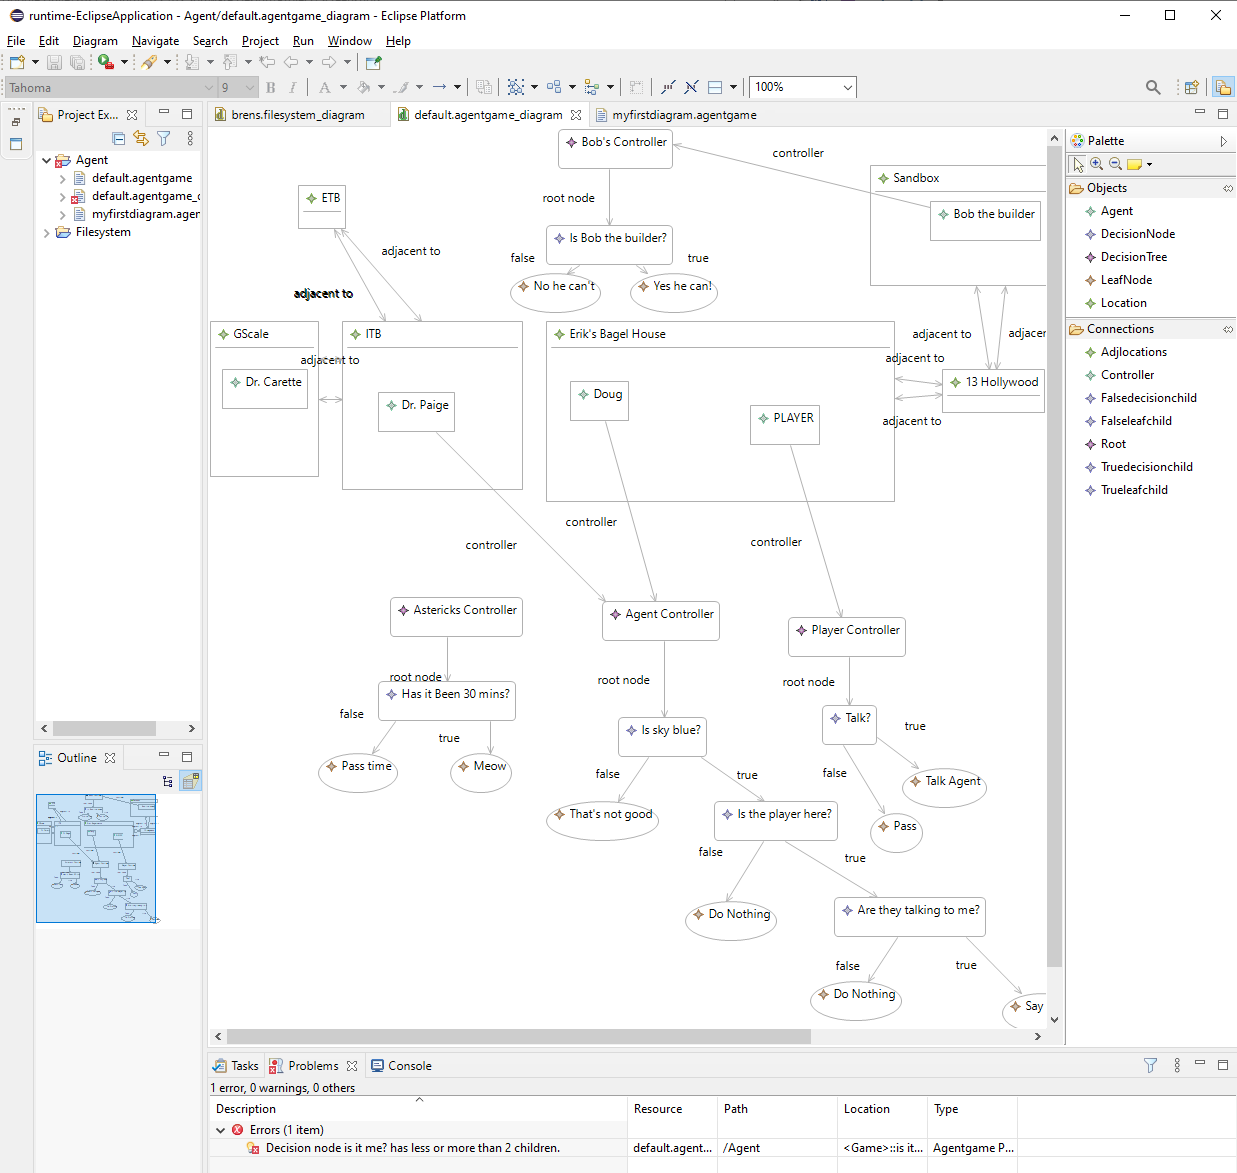
\includegraphics[width = 13 cm ]{Final Editor.png}
    \caption{The GMF-based Eugenia editor for agentgame metamodel.}
    \label{fig:editor}
\end{figure}

\subsection{Design Decisions & Strengths}
Seeing that a big proportion of the agent behaviour specification would be tree-based it makes sense to draw trees as diagrams, which is almost always done in computer science for visualization. As well, the intended userbase for the editor would be game designers that wouldn’t necessarily be that adept at textual syntaxes. Providing an easy-to-understand graphical interface would be much more intuitive for the users. Finally, laying out game objects such as locations, agents, and items also makes sense the most sense graphically. Game editors such as Unity use a 3D view for showing what the player will see and a text editor for scripting \cite{technologies_unity_nodate}.

The shapes of the symbols are important too. I wanted to do ovals for the leaf nodes as flowchart processes are usually ovals or circles. This semantic transparency also applies to the sequencing of the tree with arrows going downward. Adjacent locations have bidirectional arrows, decision trees have a line to the agent, and agents are placed in locations are examples of how the concrete syntax makes the editor intuitive to use. As such, I had to structure my metamodel accordingly so it could work with Eugenia. I wanted an arrow to denote a containment relationship between nodes but neither Eugenia phantom nodes nor affix nodes would work without disappearing. As such, I had to change the abstract syntax to associations.

\subsection{Weaknesses & fixes}
One of the biggest drawbacks of a graphical editor is visual complexity explosion. As the models get bigger and more complex than the one shown in figure \ref{fig:editor} it begins to get hard to read. The number of arrows, layout between the objects, and scrolling through a huge model would make it unusable. This lack of diagrams scaling well is a problem for a game agent designer where the behaviour trees can be very complex. As discussed in class one of the best ways to deal with this problem is modularity/chunking. Making views with only 7 +/- 2 things on them at a time may seem difficult but having specific scenes you jump between is common in game design. Having the editor be able to group and jump to different scenes with links across them would be helpful. Another method is to use hierarchy, such as making collapsing trees into a single node. If the editor could group and collapse tree diagrams it would be very helpful. It can already do this with compartments so maybe having the controller be a compartment would help with the readability of these diagrams as they get more complex.


\section{EVL Constraints}
\subsection{EVL Constraints}

Constraints are a key design choice to be able to make sure the model constructed is well-formed. As discussed in the previous section, having multiplicities on items is one constraint that limits many undesirable models already. However, UMF is lacking in its ability to define more complex constraints so we use the Epsilon model management tool. Specifically, we use the Epsilon Validation Language (EVL) to make sure any constraints needed, that aren’t covered by multiplicities, are enforced.

For my metamodel, there were 5 key constraints and 1 critique that were implemented. The following is a list of those constraints and critiques.
1. All elements must have names. This is so they are readable and distinguishable. A name for a decision node may briefly describe the logic to be implemented. I implemented this by having each class check that the name attribute was defined. If an element is unnamed it will be flagged with an error message until renamed.
2.  Decision Trees must have a root node. While the root node multiplicity is 1 that doesn’t mean that the user would attach any elements. EVL checks for this by seeing that the $root_node$ attribute is defined. If it isn’t, the quick fix will give a menu to select a decision node to be the root. An error message is thrown until this is fixed
3. A decision node must only have two children. Although it’s supposed to be a binary tree there are four possible connections each with a multiplicity of one. This constraint counts all the defined relationship and makes sure there’s only 2 defined. A node with more or less than 2 relationships will give an error with a message.
4. A decision node should only have one true child and one false child node. There is a guard to make sure the “TwoChildren” constraint has passed but these children could be any binary combination of the 4 relationship types. To enforce this constraint we can do a logical XOR of the true children, an XOR of the false children, and then logical AND those results. This XOR AND XOR check makes sure only one of each true child and false child relationship is defined. The error message states this if the decision node does not follow this rule.
5. A location can’t be adjacent to itself. Adjacency implies a separate physical entity so it wouldn’t make sense if a location was next to itself. The constraint checks all the adjacent locations in each location and makes sure none of them is the location itself. If it is, an error will be thrown until this connection is removed.
6. Critique: Agents, locations, and decision trees should have unique names. Assuming the “HasName” constraint has passed, this critique checks that no other entity of that type has the same name. This is simply to avoid confusion in naming. Duplicate game elements are completely valid and the critique can be ignored if such a case exists.

Some other constraints outside the scope of the model are making sure that decision nodes always have conditional logic and that player input is well-formed to the player controller.


\subsection{GMF EVL Integration}
The implementation of these constraints into the GMF editor was a bit more complex than I originally thought. To do this you have to make an Eclipse plugin and edit the MANIFEST.MF file to referencing the proper components and build with the EVL file. Once integrated you can launch the editor and go to edit $->$ validate to run the constraints against the model. Any update to the constraints and the editor must be relaunched. There is a tutorial on this process \cite{noauthor_live_nodate} but it isn’t the most straightforward for beginners. I had to look up a lot of secondary information that could have been included in the tutorial \cite{noauthor_eclipse_nodate}.
%As such, I decided to make my own tutorial with step-by-step pictures as seen in appendix_.

\begin{figure}[h]  % h for here, p for separate page, b\t, or !
    \centering  % centers the figure in the page
    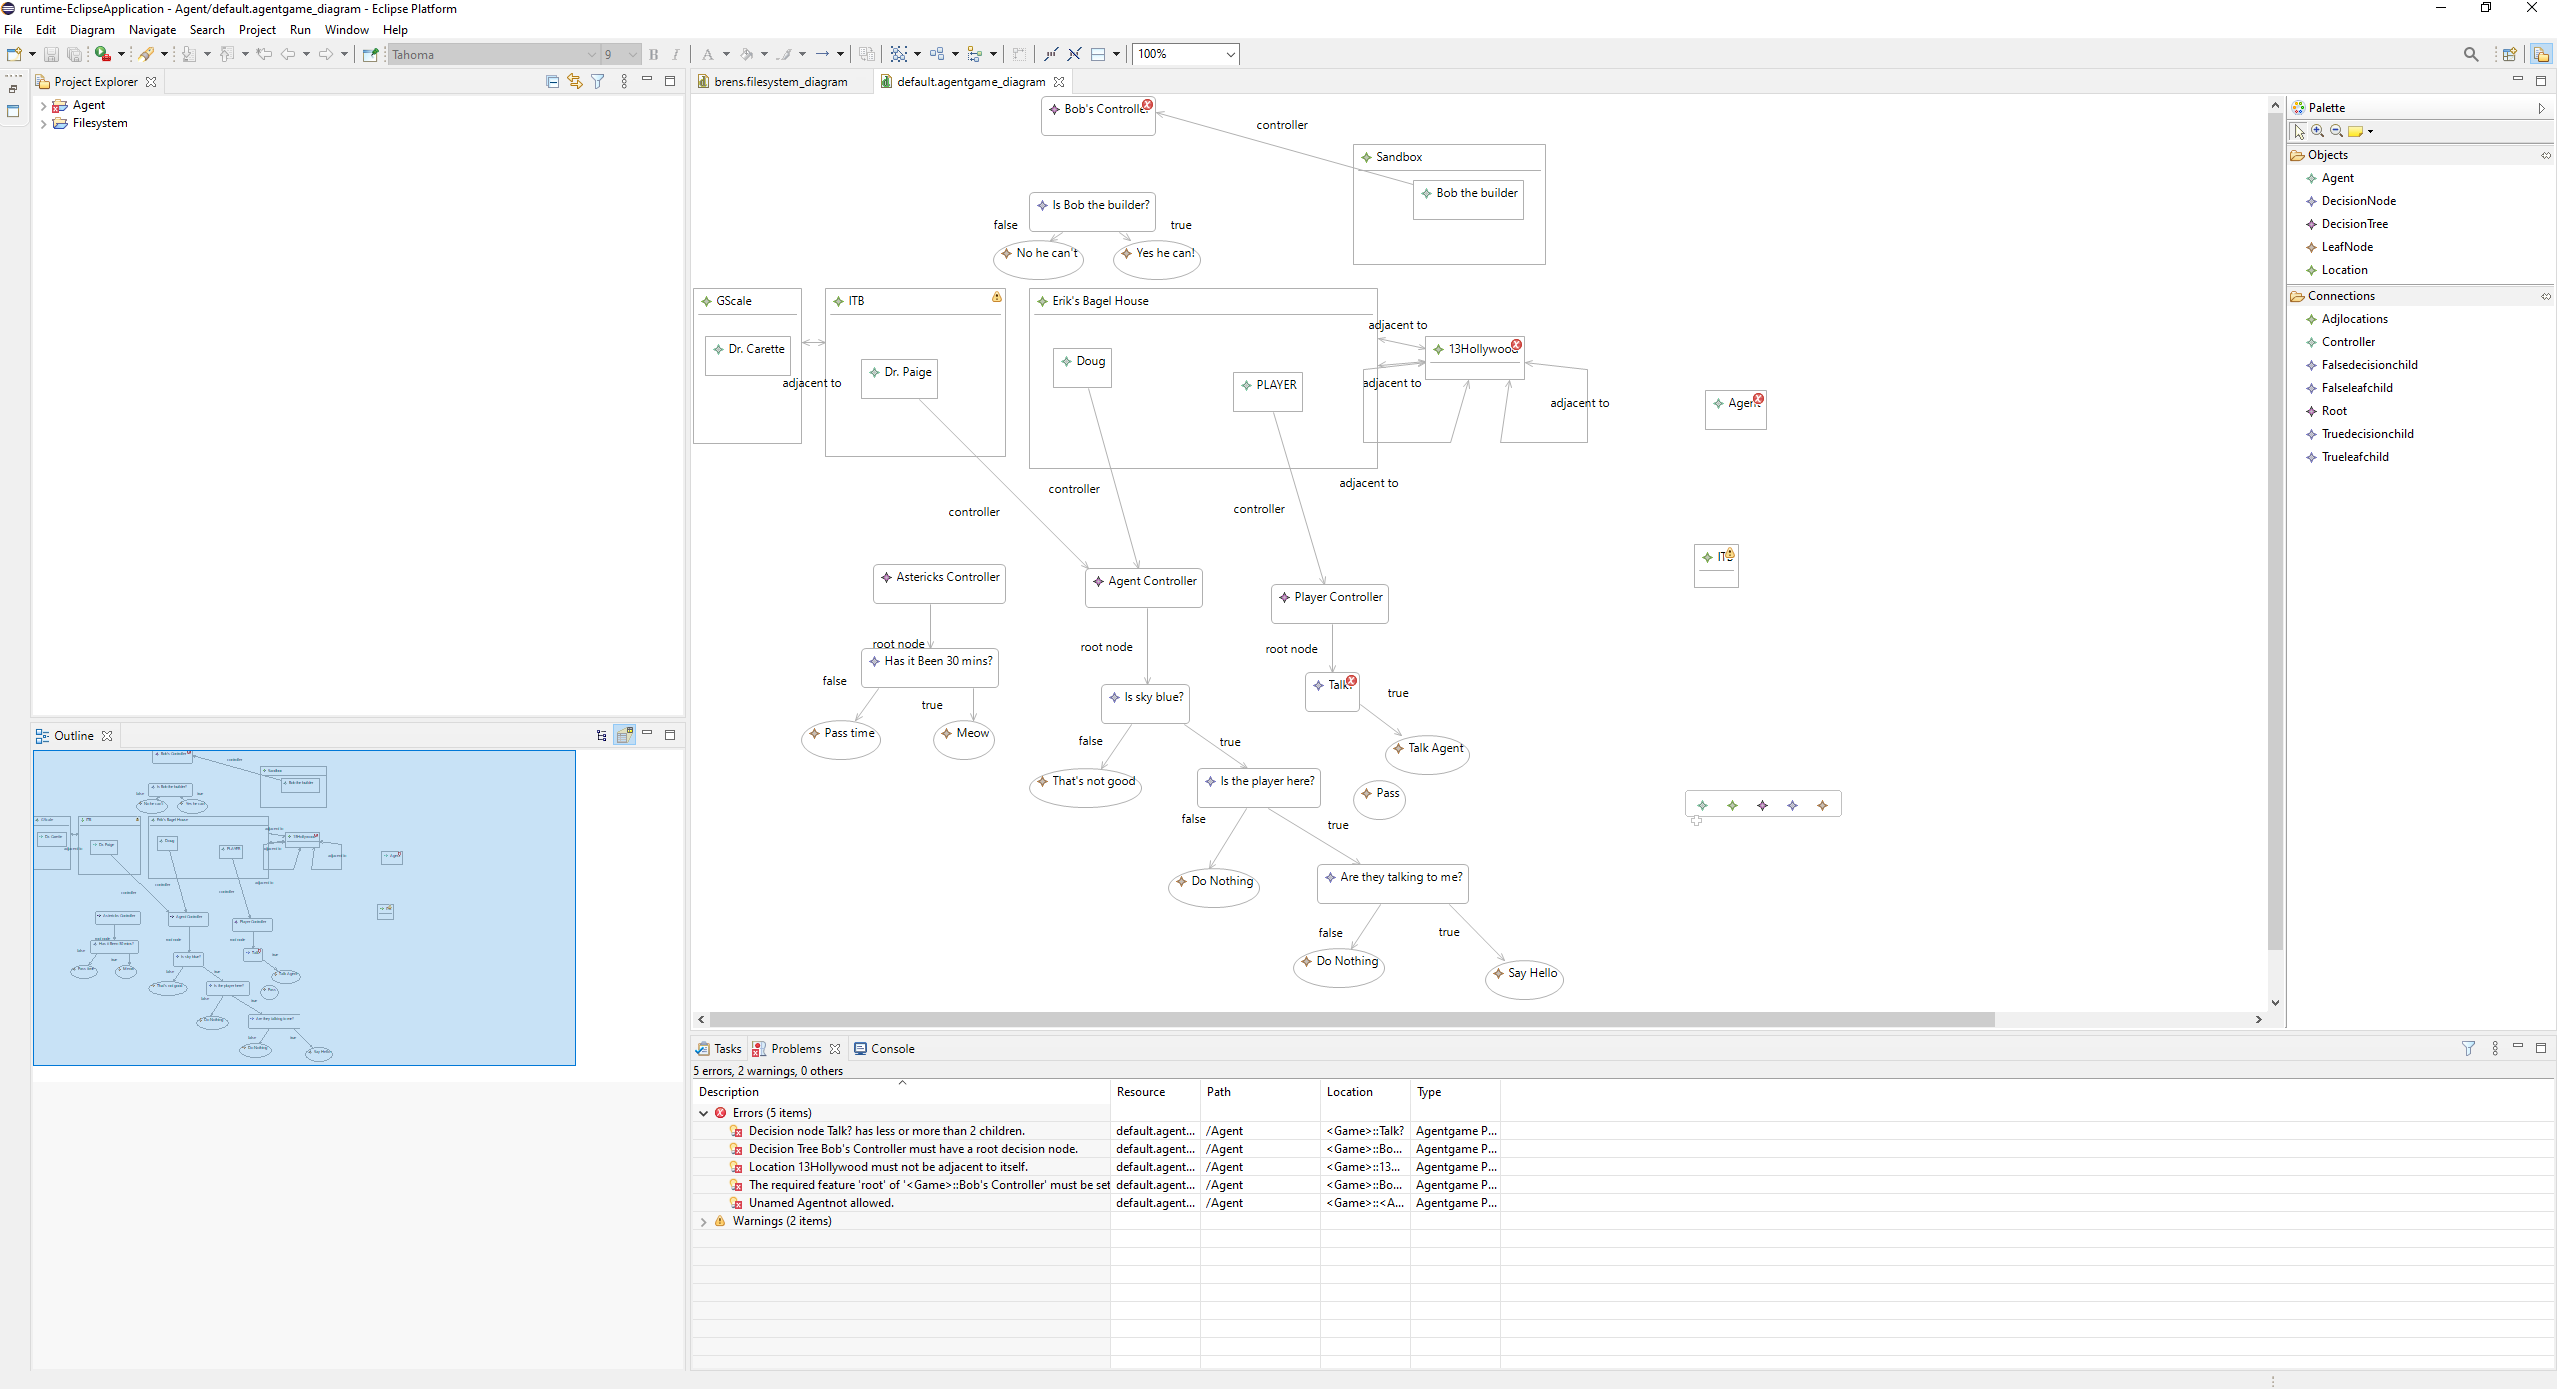
\includegraphics[width = 12 cm ]{Editor with Constraints.png}
    \caption{Editor with errors showing after validation is completed.}
    \label{fig:errors}
\end{figure}

\newpage
\section{M2T Python Code Generation}
So to create a set of game objects to be used in a game the transformation will have to be a model-to-text (M2T) transformation. Using Epsilon this can be done by using the template-based Epsilon Generation Language (EGL) with the rule-based EGX coordination language.

\subsection{Design Choices}
There were several key design choices I decided to make with this transformation. I decided to not integrate the transformation because I couldn’t find any documentation on integrating EGX with a GMF editor. I’m sure there is a way to do it with a plugin but I felt it would be much more convenient to work through the main Eclipse editor. Model management operations such as generating code may be more of a programmer domain than a game designer domain anyways. However, this means there’s no guarantee that the model is validated before it’s transformed which is a systematic flaw. To overcome this I had to add redundancies in the transformation code. I also decided to link the editor agentgame XMI file (external to the repository) to run the transformations. This means it’s running directly against the editor XMI file so any saved changes to the model will be updated in our transformations, i.e. no copying files or relaunching editors. To make it easier to reference I’ve decided to include a static model ($example_editor_diagram.agentgame$) in the project files which I will be working from as my generated example

The code generation choice to use Python was due to familiarity. Although integrating into a game engine like Unity with C# scripts would be the end goal it’s outside the scope of the project. I started by writing code in Python that I could use as a template for my EGL template. The EGX file runs each game element, i.e. the entire model, once to generate the static Python classes and object elements in a separate file. This is to cleanly separate the class code from the initialized variables.

\subsection{Challenges}
The first challenge I encounter is Python identifiers. The model name attribute wouldn’t do because anything can be typed as a name but Python variables can only be composed of underscores, characters, and numbers. I decided to follow the XMI scheme and name the variable by order of appearance in the list. I deemed this much easier to deal with than doing EOL string manipulation and testing for edge cases.

\subsubsection{Hand Written Code Integration}
One of the biggest challenges I wrestled with was how to design generated code that integrated nicely with hand-written code. In class, we covered 4 distinct methods with the simplest being protected regions or tool-integration, i.e. code imports. I went with tool integration so that the generated code and hand-written code were cleanly separated and programmers didn’t need to search through a giant generated file. The main issue was then how to structure my classes to integrate nicely between the two stages of code. Ideally, code that’s generated could be overwritten with hand-written attributes and methods. How to initialize these classes so they could reference each other and then be extended is a problem I’ve wrestled with before and didn’t know how to easily solve. To add on top of this the hand-written information to write for decision and leaf nodes would be dynamic logic instead of static references.

To overcome this extensibility challenge I decided to take advantage of higher-order functions in Python. This means I could generate an abstract class with methods that accepted functions as input. Then I could write the actual methods by hand and pass them into the objects. I did this by creating a class that copies the attributes of the abstract object into a finished class. Then to invoke the higher-order function on your data you initialize the finished class and pass logic functions.
An example is shown in appendix \ref{appendix:pythoncode} using DecisionNodes and the gotochild function.


This method is very tedious in rewriting code so it's a very DRY (don't repeat yourself) solution\cite{noauthor_dont_2021}. Having to re-write the entire class doesn't make much sense but it does cleanly separate the code. In retrospect, I would rather have just generated code and use protected sections to write the behavioural logic. This would lead to much less repeated code. I'm also sure there's a much more DRY method in Python to overwrite initialized abstract functions. That solution would be the best of both worlds.



%\section{Future Work}


\section{Conclusion}
To aid game designers a more abstract domain-specific language for specifying NPC agents was created using the Eclipse Modelling Framework. A metamodel abstract syntax was defined in Ecore/Emfatic, a graphical concrete syntax was defined using GMF/Eugenia, EVL model constraints were integrated into that editor, and a model-to-text transformation into Python code was performed taking into account extension with hand-written code.

This project was an exercise in learning the technology so the scope was very restricted. There is a lot of further work that could be done on this project including polishing the editor, adding more complex game elements, and adding better internal and external tool integration.
However, the design decisions, technologies, and concepts learned were invaluable to understanding not only model-driven engineering but software design in general.
Based on my experience making this DSL I’m hoping I can make better tools for future designers, of all levels and crafts, to create the things they love.



\addcontentsline{toc}{section}{References}  % adds a line to the table of contents, not done automatically
\bibliographystyle{plain}  % the style setup
%Enter the .bib style, can be plain or Plainnat with the nat package, can enter multiple filenames with coma
\bibliography{citations.bib}

\newpage
\appendix  % adding an appendix

%\section{Appendix: The files}
%\label{appendix:files}  % section for reference
%This is the Appendix

%\section{Appendix: Project evolution}
%\label{appendix:files}  % section for reference
%The project evolved over various stages and ideas based on limiting scope/complexity, time constraints, technology limitations, etc. I included a few screenshots on %how the modelling process evolved.

%\section{Appendix: GMF EVL Integration Tutorial}
%\label{appendix:tutorial}  % section for reference


\section{Appendix: Extending Generated Python Code Example}
\label{appendix:pythoncode}  % section for reference




\begin{figure}[h]  % h for here, p for separate page, b\t, or !
    \centering  % centers the figure in the page
    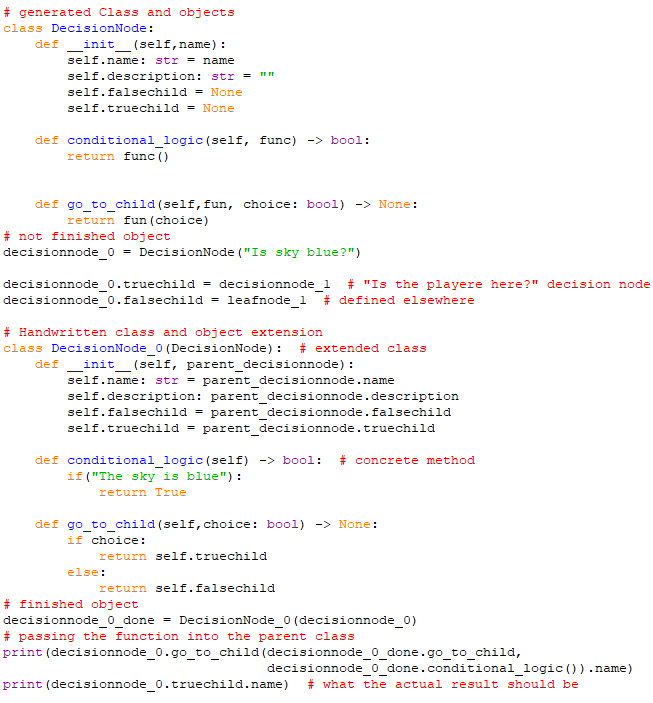
\includegraphics[width = 15 cm ]{Generated Code Extension Example.png}
    %\caption{Extending generated Python code using high-order functions.}
    \label{fig:code}
\end{figure}

%Using hand-written Python code to overwrite initialized generated code using high-order functions.



\end{document}

